\documentclass[a4paper,12pt]{article} % тип документа

% Поля страниц
\usepackage[left=2.5cm,right=2.5cm,
    top=2cm,bottom=2cm,bindingoffset=0cm]{geometry}
 
    
%Отступ после заголовка    
\usepackage{indentfirst}


% Рисунки
\usepackage{floatrow,graphicx,calc}
\usepackage{wrapfig}

% Создаёем новый разделитель
\DeclareFloatSeparators{mysep}{\hspace{1cm}}

% Ссылки?
\usepackage{hyperref}
\usepackage[rgb]{xcolor}
\hypersetup{				% Гиперссылки
    colorlinks=true,       	% false: ссылки в рамках
	urlcolor=blue          % на URL
}


%  Русский язык
\usepackage[T2A]{fontenc}			% кодировка
\usepackage[utf8]{inputenc}			% кодировка исходного текста
\usepackage[english,russian]{babel}	% локализация и переносы


% Математика
\usepackage{amsmath,amsfonts,amssymb,amsthm,mathtools}


% Что-то 
\usepackage{wasysym}


%Заговолок
\author{Серебренников Даниил Б02-826}
\title{Лабораторная работа \No 2.2.3}


\begin{document}


\begin{center}
\footnotesize{ФЕДЕРАЛЬНОЕ ГОСУДАРСТВЕННОЕ АВТОНОМНОЕ ОБРАЗОВАТЕЛЬНОЕ 			УЧРЕЖДЕНИЕ ВЫСШЕГО ОБРАЗОВАНИЯ}\\
\footnotesize{МОСКОВСКИЙ ФИЗИКО-ТЕХНИЧЕСКИЙ ИНСТИТУТ\\(НАЦИОНАЛЬНЫЙ 			ИССЛЕДОВАТЕЛЬСКИЙ УНИВЕРСИТЕТ)}\\
\footnotesize{ФАКУЛЬТЕТ ОБЩЕЙ И ПРИКЛАДНОЙ ФИЗИКИ\\}
\hfill \break
\hfill\break
\hfill\break
\hfill \break
\hfill \break
\hfill \break
\hfill \break
\hfill \break
\hfill \break
\hfill \break
\hfill \break
\hfill \break
\hfill \break
\hfill \break
\hfill \break
\large{Лабораторная работа № 2.2.3\\\textbf{Определение теплопроводности газов	\\при атмосферном давлении}}\\
\hfill \break
\hfill \break
\hfill \break
\begin{flushright}
	Серебренников Даниил\\
	Группа Б02-826
\end{flushright}
\hfill \break
\hfill \break
\hfill \break
\hfill \break
\hfill \break
\end{center}
\hfill \break
\hfill \break
\hfill \break
\hfill \break
\hfill \break
\begin{center}
	Долгопрудный, 2019 г.
\end{center}
\thispagestyle{empty} % выключаем отображение номера для этой страницы


\newpage
\textbf{Цель работы:} определение коэффициента теплопроводности воздуха при атмосферном давлении и разных температурах по теплоотдаче нагреваемой током нити в цилиндрическом сосуде.

\textbf{В работе используются:} прибор для опредления теплопроводности газов; форвакуумный насос; газгольдер с газом; манометр; магазин сопротивлений; эталонное сопротивление 10 Ом; цифровой вольтметр B7-78/1; источник питания.


\section{Теоретическая часть}

	Основной характеристикой теплопроводности служит коэффициент $\varkappa$, являющийся коэффициентом пропорциональности между плотностью потока тепла $q$ и градиентом температуры $dT/dr$ в направлении распространения этого потока
\begin{equation}
	q = -\varkappa \frac{dT}{dr}.
\end{equation}

	В цилиндрически симметричной установке, в которой тепловой поток направлен к стенкам цилиндра от нити, полынй поток тепла $Q = qS$ через каждую цилиндрическую поверхность радиуса $r$ должен в стационарном состоянии быть неизменен (как в пространстве, так и во времени). Тогда
\begin{equation}
	Q = -2\pi rL\varkappa \frac{dT}{dr} = const,	
\end{equation}
откуда получаем формулу
\begin{equation}
	\label{formula}
	T_1 - T_2 = \frac{Q}{2\pi L\varkappa} \ln \frac{r_2}{r_1}.
\end{equation}
Здесь $r_1$ и $T_1$ -- радиус и температура нити, $r_2$ и $T_2$ -- радиус и температура цилиндра.


\section{Экспериментальная установка}

	Схема установки изображена на рис.~\ref{ris:ustanovka}. Тонкая молибденовая нить натянута по оси длинной вертикально стоящей медной трубки\footnote{В нашей установке диаметр проволоки $2r_1 \approx 0,055$ мм, внутренний диаметр трубки $2r_2 \approx 10$ мм, длина $L \approx 355$ мм.}.
	Через штуцер трубка заполняется исследуемым газом. Нить нагревается электрическим током, а её температура $T_1$ определяется по изменению электрического сопротивления. Трубка находится в кожухе, через которой пропускается вода из термостата. Температура воды $T_2$ измеряется термометром, помещенным в термостат. Количество теплоты, протекающей через газ, равно, если принебречь утечками тепла через торцы, количеству теплоты, выделяемому током в нити, и может быть найдено по закону Джоуля-Ленца\footnote{Мощность электрического тока, протекающего через нить: $Q = I^2 R$}. При этом ток в нити определяется по напряжению на включенном последовательно с ней эталонном сопротивлении $R_0 = (10,00 \pm 0,01)$ Ом.
	
	Электрическая часть схемы состоит из источника питания и подключенных к нему последовательно соединенных нити, эталонного сопротивления и магазина сопротивлений $R$, служащего для точной установки тока через нить. Цифровой вольтметр может подключаться как к нити, так и к эталонному сопротивлению, измеряя таким образом напряжение на нити и ток через неё.
	
\begin{figure}[h]
	\center{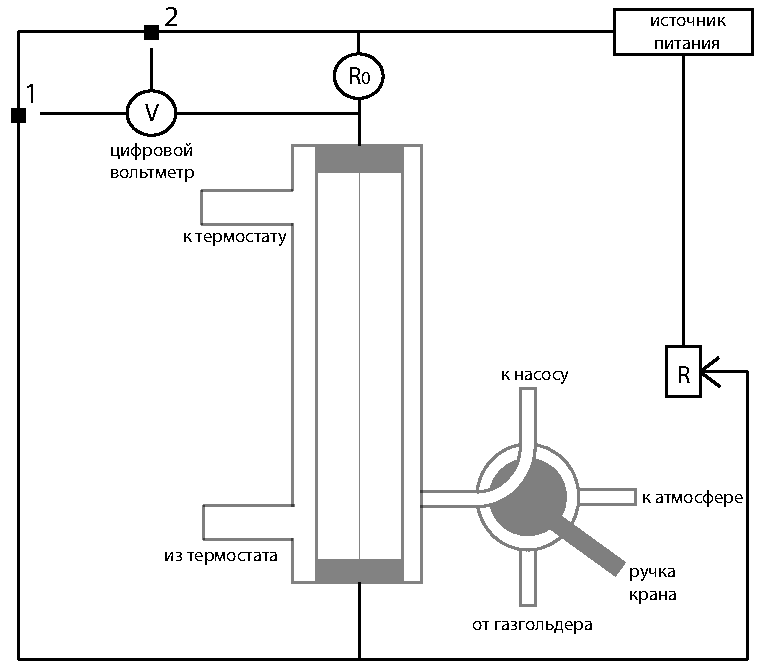
\includegraphics[scale=1]{Draw_1.pdf}}
	\caption{Схема установки для определения теплопроводности газов}
	\label{ris:ustanovka}
\end{figure}
	
	
\section{Экспериментальная часть}
\begin{enumerate}

\item
	Снимем зависимость напряжения на нити $U$ от напряжения на 	эталонном сопротивлении 	$U_0$. После изменения тока в проволоке выдержим паузу для установления стационарного 	режима.
	
\item
	Повторим измерения п. 1 ещё при температурах прибора в интервале 30--70 $^\circ$C.

\item
	Вычислим при различных токах, протекающих через нить, её сопротивление по формуле $R = R_0 \frac{U}{U_0}$ и поток тепла: $Q = \frac{U_0 U}{R_0}$. Повторим вычисления для 		всех температур прибора в этой лабораторной работе. Результаты измерений и вычислений 	представлены в таблице~\ref{table:results_1}. Оценим относительную погрешность измеренных величин: $\frac{\sigma_Q}{Q} = \frac{\sigma_R}{R} = \sqrt{(\frac{\sigma_U}{U})^2+(\frac{\sigma_U}{U_0})^2+(\frac{\sigma_{R_0}}{R_0})^2}\approx \frac{\sigma_{R_0}}{R_0} = 0,1 \%$, где $\sigma_U = 0,00005$ В, поэтому погрешностью этих величин можно пренебречь.

\item
	Для каждой температуры прибора построим график зависимости выделяемой мощности $Q$ от сопротивления нити $R$. Аппроксимацию прямой произведем методом наименьших квадратов в компьютерной программе <<OriginPro>>, в которой определим наклон $dQ/dR$ с погрешностью и сопротивление нити $R|_{Q = 0}$ при температуре термостата, то есть при нулевой выделяемой мощности. Полученные данные занесём в таблицу~\ref{table:results_2}. Графики представлены на рисунках: рис.~\ref{fig:Graph_1}, рис.~\ref{fig:Graph_2}, рис.~\ref{fig:Graph_3}, рис.~\ref{fig:Graph_4}, рис.~\ref{fig:Graph_5}, рис.~\ref{fig:Graph_6}. При расчете погрешности наклона прямой, представленной на рис.~\ref{fig:Graph_2}, мы принебрежем двумя крайними точками, которые не идеально ложатся на прямую.



\newpage
\floatsetup[table]{capposition=top}	
\begin{table}[h!]
\centering
\caption{Результаты измерений и вычислений.}
\label{table:results_1}
\begin{tabular}{|c|c|c|c|c|c|c|c|}
\hline
$T$, $^\circ$C   & \multicolumn{7}{c|}{21,4}                                           \\ \hline
$U_0$, V   & 0,1078  & 0,2088  & 0,5558  & 0,7398  & 1,1040  & 1,2690  & 1,5226  \\ \hline
$U$, V   & 0,1074  & 0,2082  & 0,5588  & 0,7493  & 1,1413  & 1,3278  & 1,6282  \\ \hline
$R$, Ohm & 9,96  & 9,97  & 10,05 & 10,13 & 10,34 & 10,46 & 10,69 \\ \hline
$Q$, W    & 0,0012  & 0,0043  & 0,0311  & 0,0554  & 0,1260  & 0,1685  & 0,2479  \\ \hline
\multicolumn{8}{|c|}{}                                                        \\ \hline
$T$, $^\circ$C   & \multicolumn{7}{c|}{30,1}                                           \\ \hline
$U_0$, V   & 0,1077  & 0,2085  & 0,5537  & 0,7362  & 1,0955  & 1,2508  & 1,6116  \\ \hline
$U$, V   & 0,1107  & 0,2145  & 0,5742  & 0,7688  & 1,1666  & 1,3550  & 1,7897  \\ \hline
$R$, Ohm & 10,28 & 10,29 & 10,37 & 10,44 & 10,65 & 10,83 & 11,12 \\ \hline
$Q$, W    & 0,0012  & 0,0045  & 0,0318  & 0,0566  & 0,1278  & 0,1695  & 0,2884  \\ \hline
\multicolumn{8}{|c|}{}                                                        \\ \hline
$T$, $^\circ$C   & \multicolumn{7}{c|}{40,0}                                           \\ \hline
$U_0$, V   & 0,1283  & 0,2083  & 0,5523  & 0,7339  & 1,0910  & 1,2516  & 1,5310  \\ \hline
$U$, V   & 0,1366  & 0,2219  & 0,5930  & 0,7930  & 1,2009  & 1,3932  & 1,7434  \\ \hline
$R$, Ohm & 10,65 & 10,65 & 10,74 & 10,81 & 11,01 & 11,13 & 11,39 \\ \hline
$Q$, W    & 0,0018  & 0,0046  & 0,0328  & 0,0582  & 0,1310  & 0,1744  & 0,2669  \\ \hline
\multicolumn{8}{|c|}{}                                                        \\ \hline
$T$, $^\circ$C   & \multicolumn{7}{c|}{50,0}                                           \\ \hline
$U_0$, V   & 0,1076  & 0,2080  & 0,5509  & 0,7311  & 1,0845  & 1,2435  & 1,5191  \\ \hline
$U$, V   & 0,1184  & 0,2292  & 0,6114  & 0,8166  & 1,2337  & 1,4295  & 1,7846  \\ \hline
$R$, Ohm & 11,00 & 11,02 & 11,10 & 11,17 & 11,38 & 11,50 & 11,75 \\ \hline
$Q$, W    & 0,0013  & 0,0048  & 0,0337  & 0,0597  & 0,1338  & 0,1778  & 0,2711  \\ \hline
\multicolumn{8}{|c|}{}                                                        \\ \hline
$T$, $^\circ$C   & \multicolumn{7}{c|}{60,0}                                           \\ \hline
$U_0$, V   & 0,1075  & 0,2078  & 0,5492  & 0,7282  & 1,0783  & 1,2582  & 1,5070  \\ \hline
$U$, V   & 0,1223  & 0,2367  & 0,6300  & 0,8405  & 1,2665  & 1,4951  & 1,8256  \\ \hline
$R$, Ohm & 11,38 & 11,39 & 11,47 & 11,54 & 11,75 & 11,88 & 12,11 \\ \hline
$Q$, W    & 0,0013  & 0,0049  & 0,0346  & 0,0612  & 0,1366  & 0,1881  & 0,2751  \\ \hline
\multicolumn{8}{|c|}{}                                                        \\ \hline
$T$, $^\circ$C   & \multicolumn{7}{c|}{70,0}                                           \\ \hline
$U_0$, V   & 0,1075  & 0,2076  & 0,5476  & 0,7254  & 1,0080  & 1,2499  & 1,4952  \\ \hline
$U$, V   & 0,1263  & 0,2441  & 0,6483  & 0,8642  & 1,2172  & 1,5314  & 1,8660  \\ \hline
$R$, Ohm & 11,75 & 11,76 & 11,84 & 11,91 & 12,08 & 12,25 & 12,48 \\ \hline
$Q$, W    & 0,0014  & 0,0051  & 0,0355  & 0,0627  & 0,1227  & 0,1914  & 0,2790  \\ \hline
\end{tabular}
\end{table}


\floatsetup[table]{capposition=top}	
\begin{table}[h!]
\caption{Результаты вычислений.}
\label{table:results_2}
\begin{tabular}{|c|c|c|c|c|c|c|}
\hline
$T$, $^\circ$C          & 21,4  & 30,1  & 40,0  & 50,0  & 60,0  & 70,0  \\ \hline
$R|_{Q = 0}$, Ohm       & 9,96  & 10,28 & 10,65 & 11,00 & 11,38 & 11,75 \\ \hline
$dQ/dR$, W/Ohm          & 0,336 & 0,341 & 0,358 & 0,363 & 0,372 & 0,379 \\ \hline
$\sigma_{dQ/dR}$, W/Ohm & 0,006 & 0,002 & 0,001 & 0,002 & 0,001 & 0,002 \\ \hline
\end{tabular}
\end{table}



\newpage
\newgeometry{bottom=2cm, left=1cm, right=1cm, top=1.5cm}	
\thisfloatsetup{floatrowsep=mysep}	
\begin{figure}[h!]
\begin{floatrow}
 \ffigbox[\FBwidth]{\caption{$Q = Q(R)$ при $T = 294$ К.}\label{fig:Graph_1}}%
         {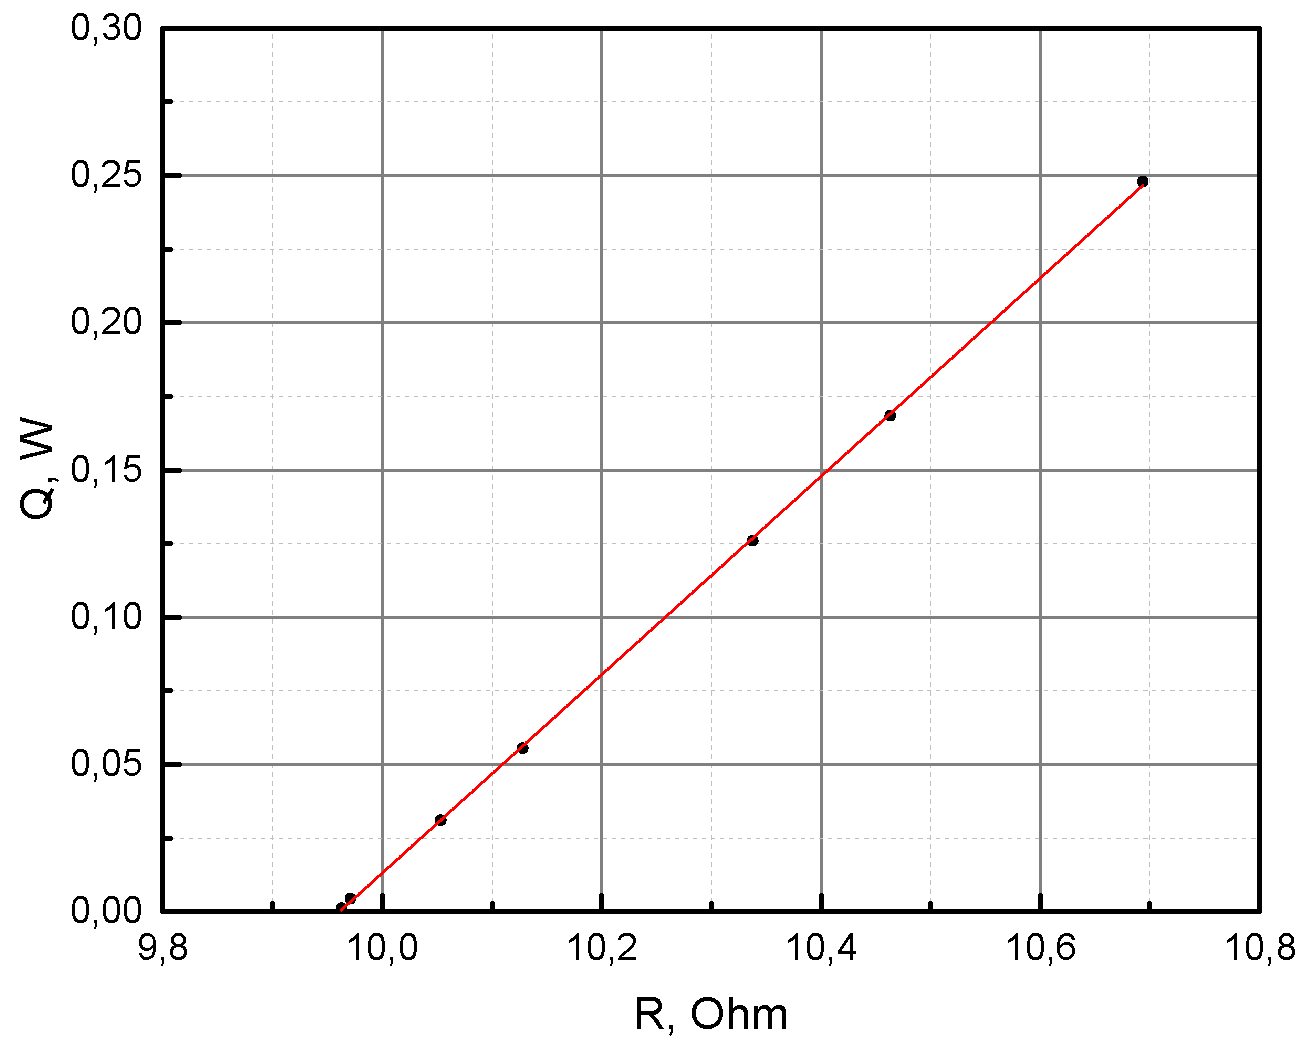
\includegraphics[width=8cm,height=7cm]{Graph_1}}
 \ffigbox[\FBwidth]{\caption{$Q = Q(R)$ при $T = 303$ К.}\label{fig:Graph_2}}%
         {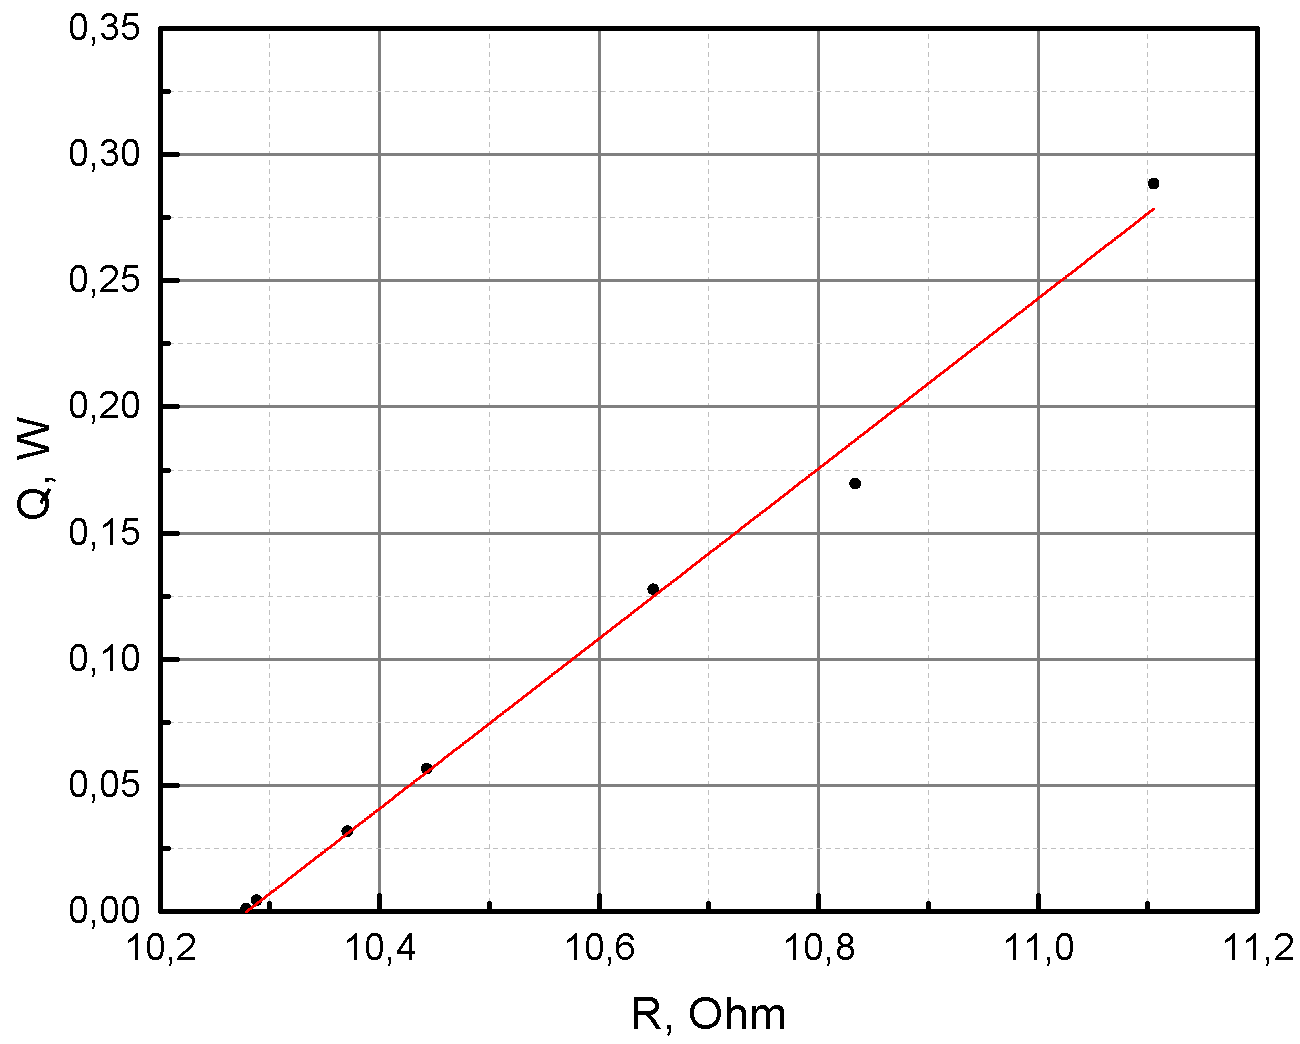
\includegraphics[width=8cm,height=7cm]{Graph_2}}         
\end{floatrow}
\end{figure}

\thisfloatsetup{floatrowsep=mysep}	
\begin{figure}[h!]
\begin{floatrow}
 \ffigbox[\FBwidth]{\caption{$Q = Q(R)$ при $T = 313$ К}\label{fig:Graph_3}}%
         {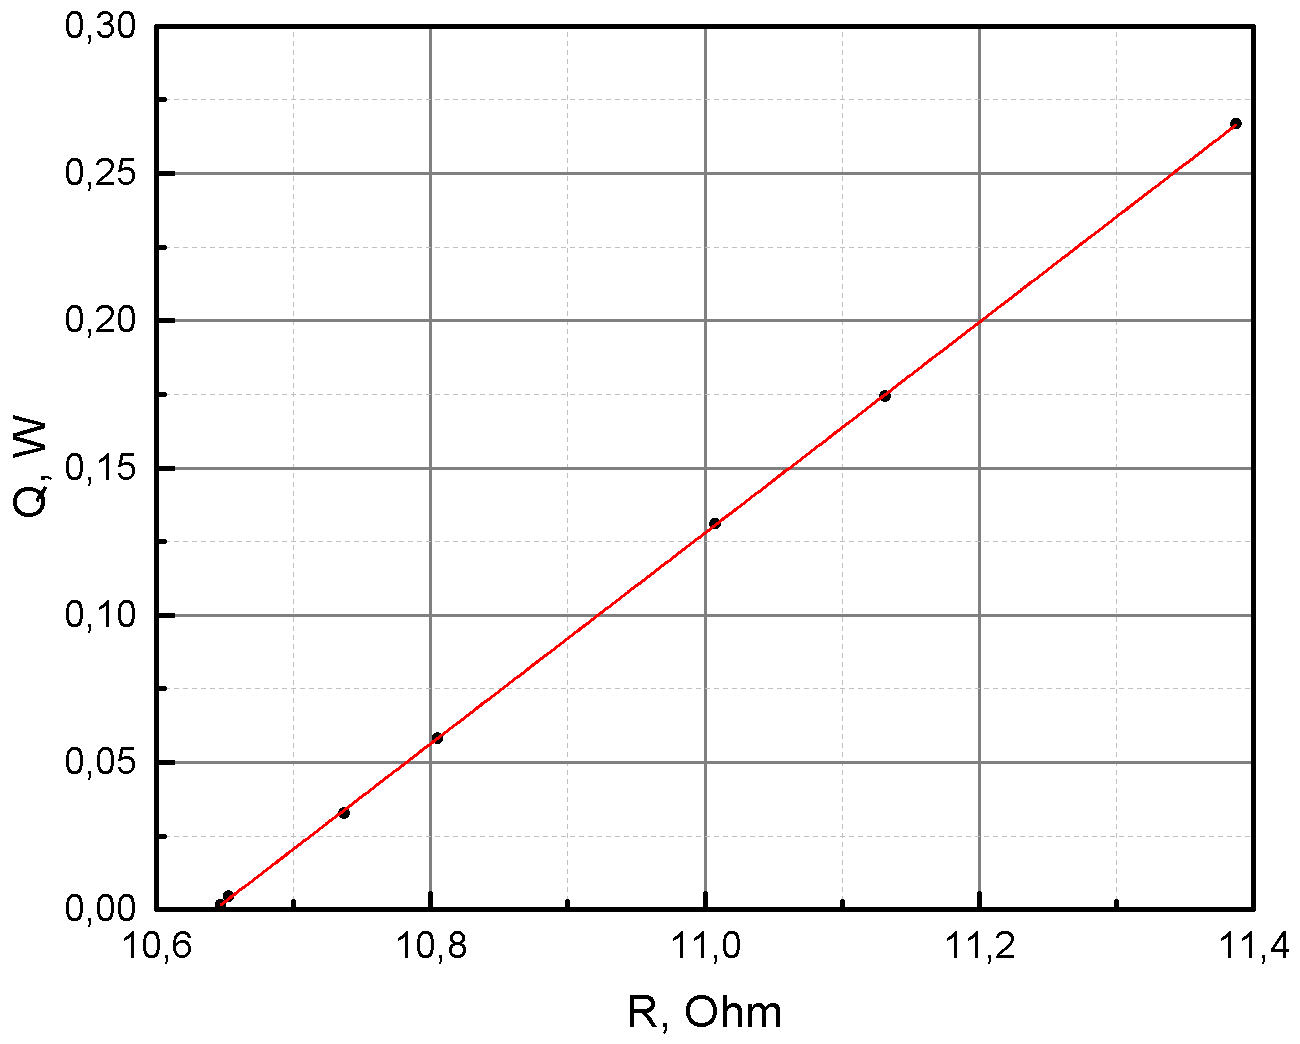
\includegraphics[width=8cm,height=7cm]{Graph_3}}
 \ffigbox[\FBwidth]{\caption{$Q = Q(R)$ при $T = 323$ К}\label{fig:Graph_4}}%
         {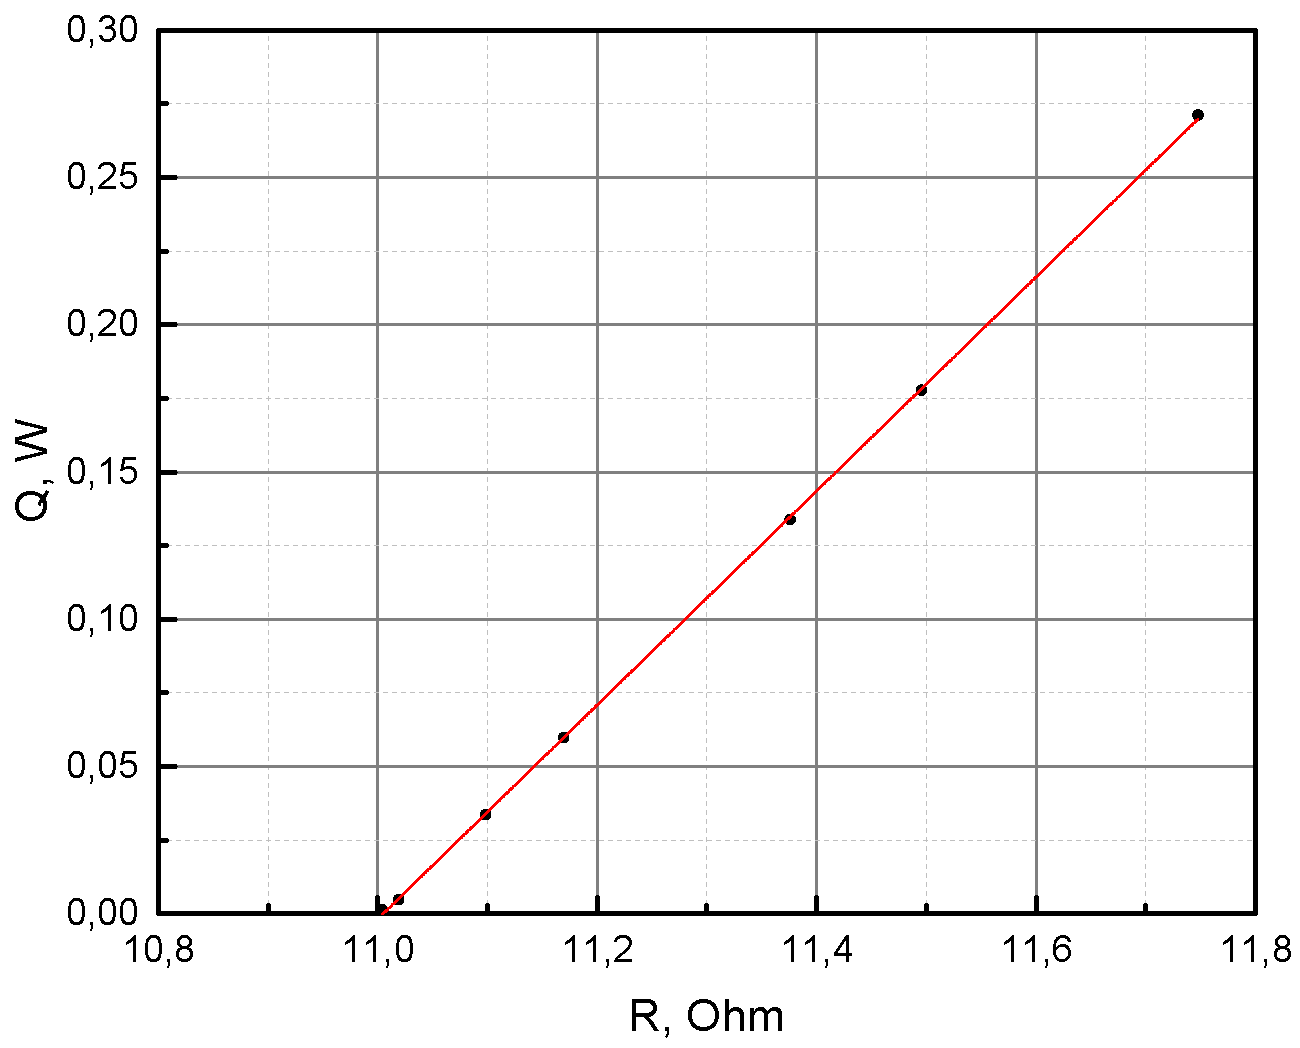
\includegraphics[width=8cm,height=7cm]{Graph_4}}         
\end{floatrow}
\end{figure}

\thisfloatsetup{floatrowsep=mysep}	
\begin{figure}[h!]
\begin{floatrow}
 \ffigbox[\FBwidth]{\caption{$Q = Q(R)$ при $T = 333$ К}\label{fig:Graph_5}}%
         {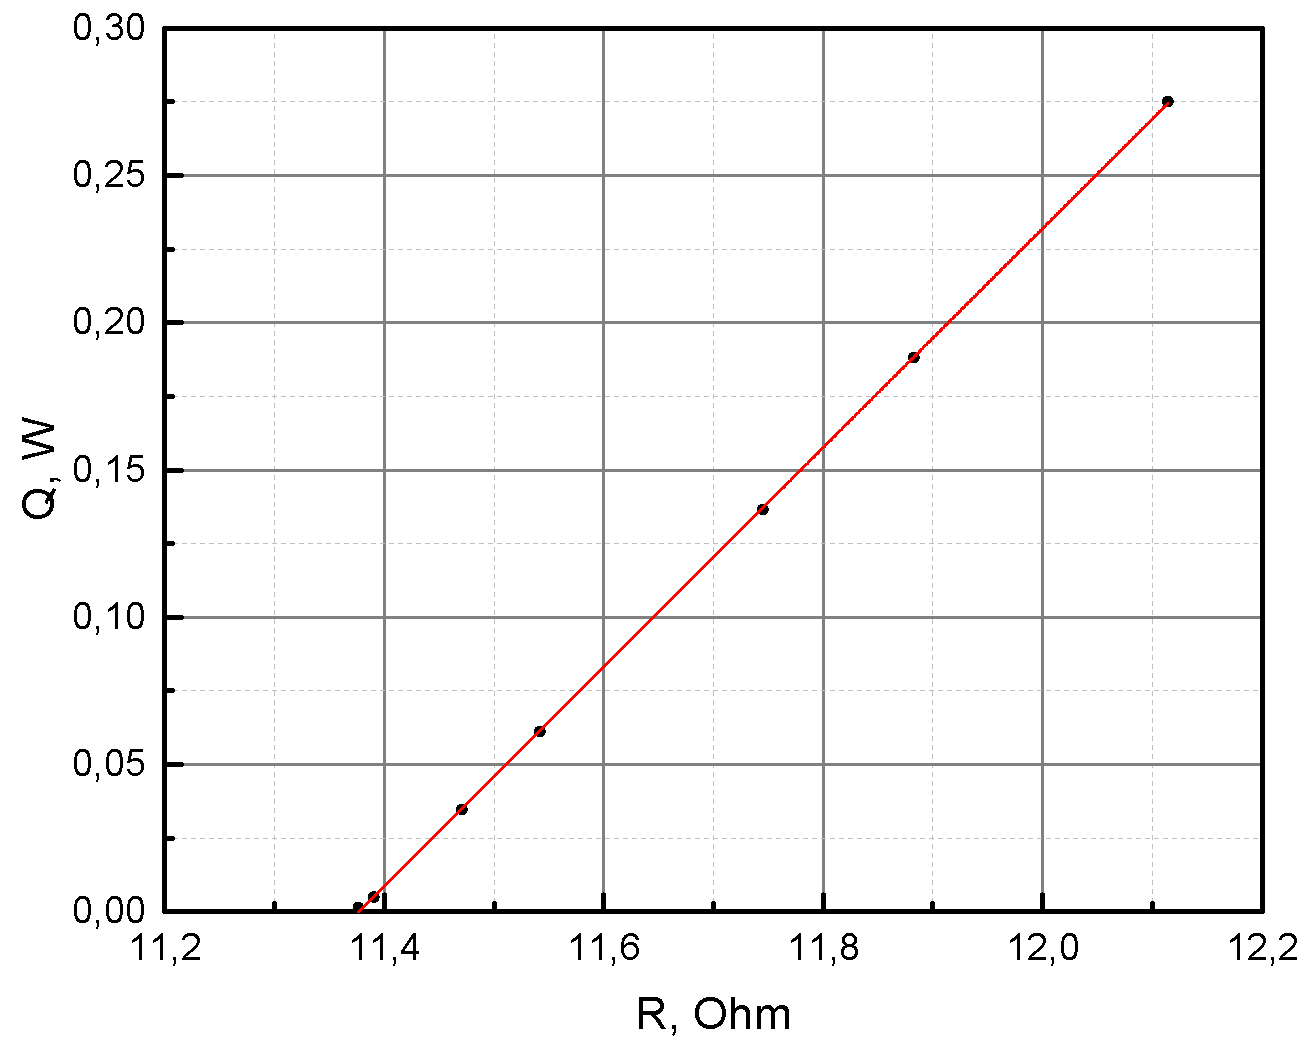
\includegraphics[width=8cm,height=7cm]{Graph_5}}
 \ffigbox[\FBwidth]{\caption{$Q = Q(R)$ при $T = 343$ К}\label{fig:Graph_6}}%
         {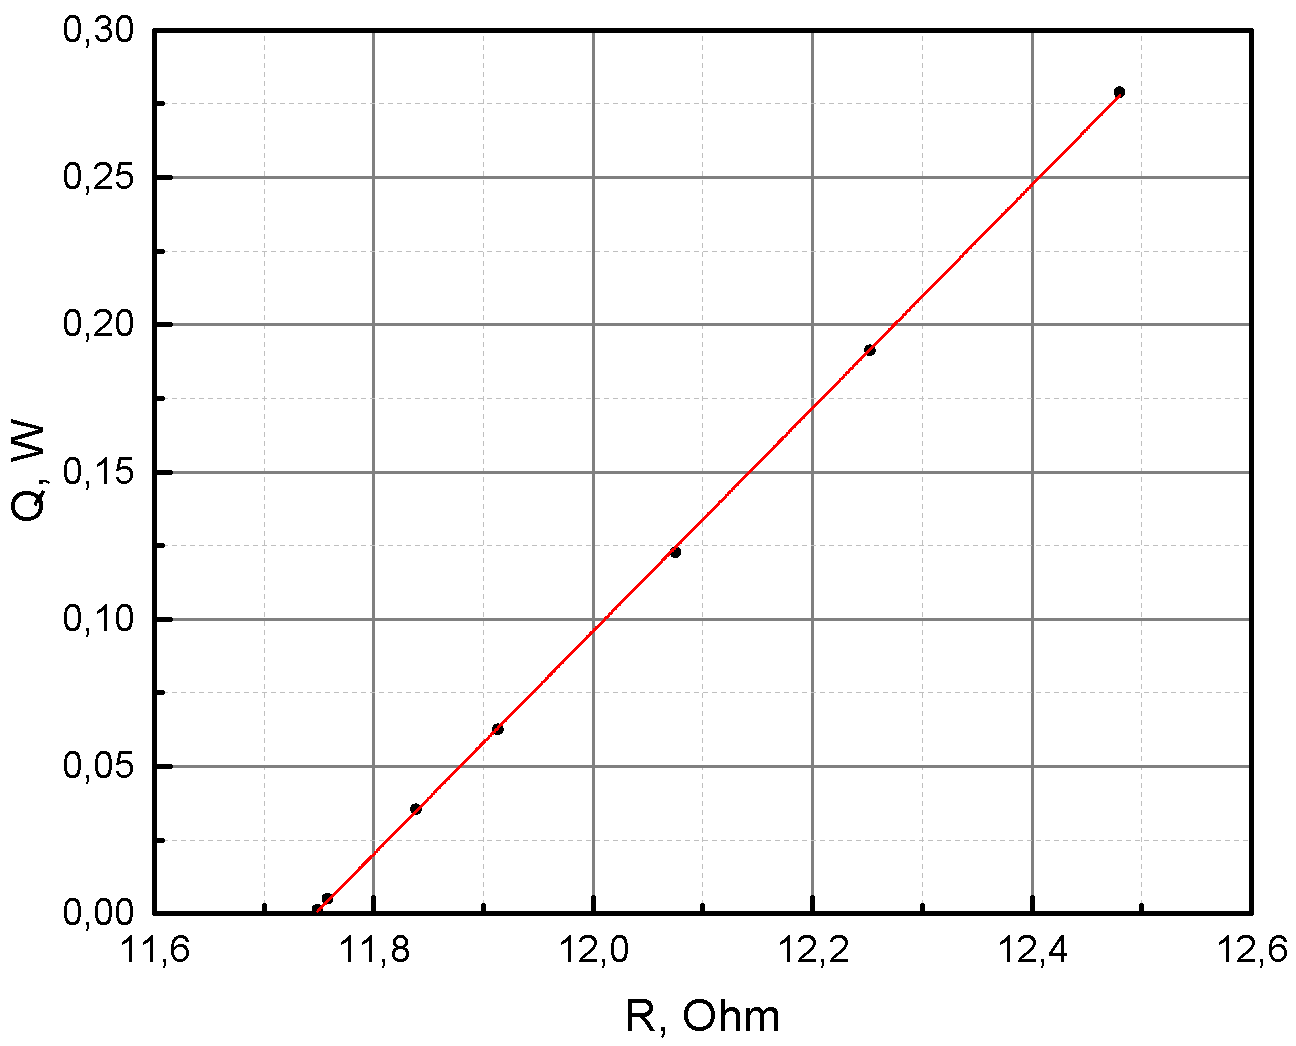
\includegraphics[width=8cm,height=7cm]{Graph_6}}         
\end{floatrow}
\end{figure}
\restoregeometry



\newpage	
\item
	Построим по значениям $R|_{Q = 0}$ график (рис.~\ref{ris:Graph_7}) зависимости сопротивления нити от температуры $T$. Апроксимацию прямой и расчет наклона $dR/dT$ произведем аналогично п. 4.
	%, а затем рассчитаем температурный коэффициент сопротивления материала нити $\alpha = \frac{1}{R_{273}} \frac{dR}{dT}$, где $R_{273} = \rho \frac{L}{\pi r_1^2}$ -- сопротивление молибденовой нити при $0$ $^\circ$C. Будем считать известным удельное сопротивление молибдена при $0$ $^\circ$C $\rho = 5,17 \cdot 10^{-8}$ Ohm$\cdot$m.
	
\begin{figure}[h]
	\center{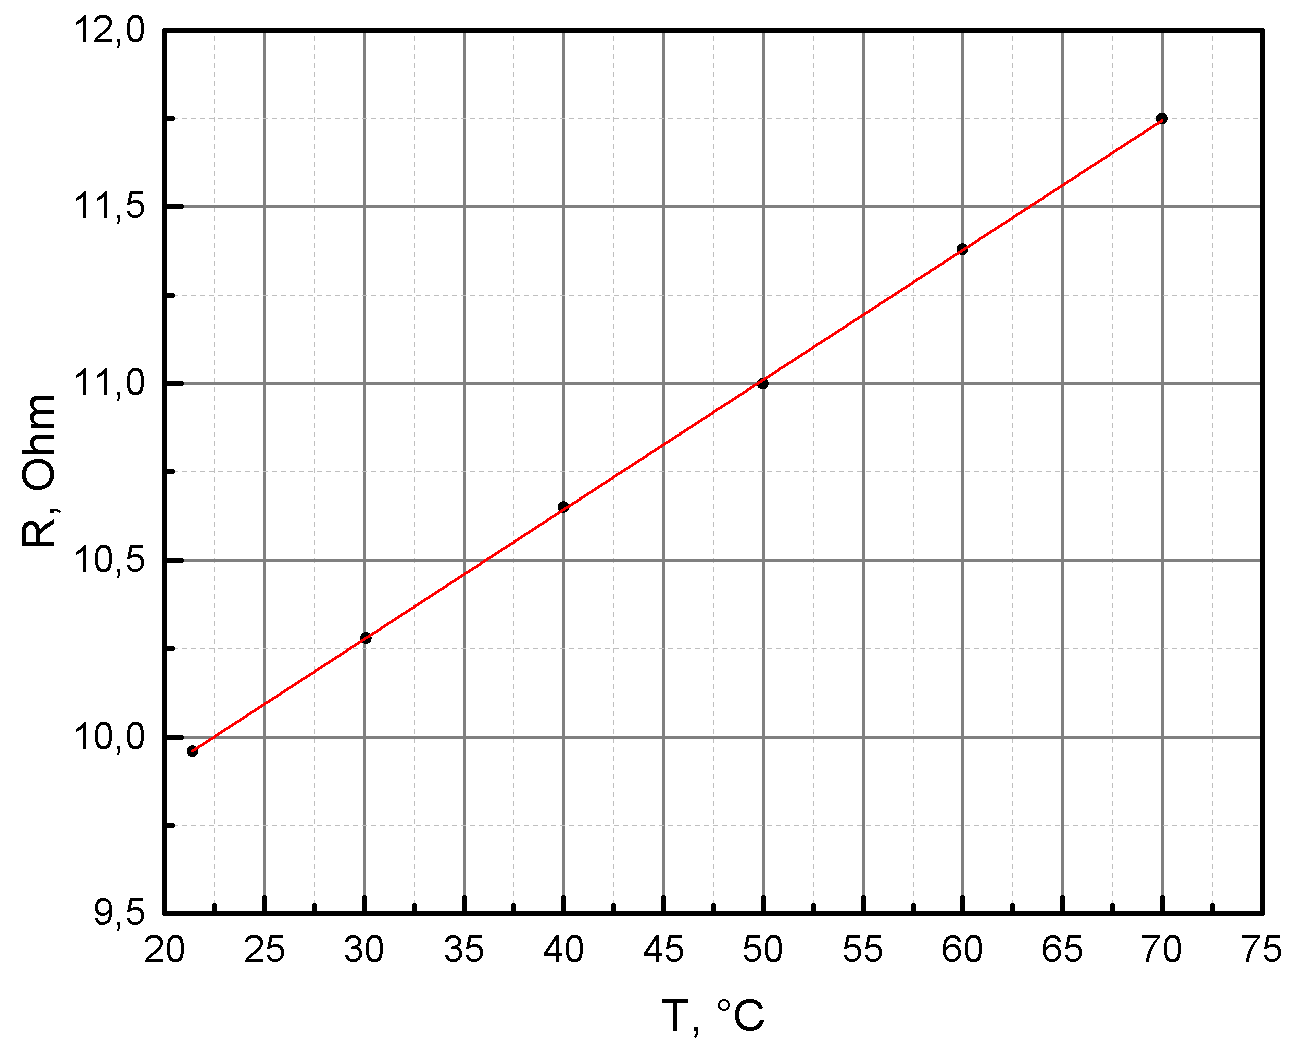
\includegraphics[scale=0.5]{Graph_7.pdf}}
	\caption{$R = R(T)$}
	\label{ris:Graph_7}
\end{figure}

	Экспериментальные точки отлично ложатся на прямую, имеющую наклон: $dR/dT = (0,0367 \pm 0,0001)$ Ohm/K.
	%Температурный коэффициент сопротивления материала нити $\alpha = 4,75 \cdot 10^{-3}$ Ohm/K.

	
\item
	Для каждой температуры прибора определим значение коэффициента теплопроводности газа по формуле $\varkappa = \frac{dQ}{dR} \frac{dR}{dT} \frac{1}{2\pi L} \ln \frac{r_2}{r_1}$. Предполагая, что зависимость коэффициента теплопроводности от температуры имеет вид $\varkappa = AT^\beta$, по полученным значениям построим апроксимированную кривую рис.~\ref{fig:Graph_8_1}. Чтобы определить показатель степени $\beta$ построим график зависимости $\ln {\frac{\varkappa}{\varkappa_0}}$ от $\ln {\frac{T}{T_0}}$, где $\varkappa_0 = 25,9$ mW/(m$\cdot$K) -- табличное значение теплопроводности воздуха при температуре $T_0 = 293$ К. Результаты вычислений представлены в таблице~\ref{table:results_3}.
	
	
\floatsetup[table]{capposition=top}	
\begin{table}[h]
\caption{Результаты вычислений.}
\label{table:results_3}
\begin{tabular}{|c|c|c|c|c|c|c|}
\hline
T, K                                  & 294,4  & 303,1  & 313,0  & 323,0  & 333,0  & 343,0  \\ \hline
$\varkappa$, mW/(Ohm*K)               & 28,8   & 29,2   & 30,6   & 31,1   & 31,8   & 32,4   \\ \hline
$\sigma_{\varkappa}$, mW/(Ohm*K)      & 0,5    & 0,2    & 0,1    & 0,2    & 0,1    & 0,2    \\ \hline
$\ln {T/T_0}$                         & 0,0048 & 0,0340 & 0,0660 & 0,0975 & 0,1280 & 0,1576 \\ \hline
$\ln {\varkappa/\varkappa_0}$         & 0,106  & 0,120  & 0,167  & 0,183  & 0,205  & 0,224  \\ \hline
$\sigma_{\ln {\varkappa/\varkappa_0}}$ & 0,017  & 0,007  & 0,003  & 0,006  & 0,003  & 0,006  \\ \hline
\end{tabular}
\end{table}


Аппроксимацию прямой (рис.~\ref{fig:Graph_8_2}) произведем методом наименьших квадратов в компьютерной программе <<OriginPro>>. Имеем: $\beta = 0,73 \pm 0,08$.


\thisfloatsetup{floatrowsep=mysep}	
\begin{figure}[h!]
\begin{floatrow}
 \ffigbox[\FBwidth]{\caption{$\varkappa = \varkappa(T)$.}\label{fig:Graph_8_1}}%
         {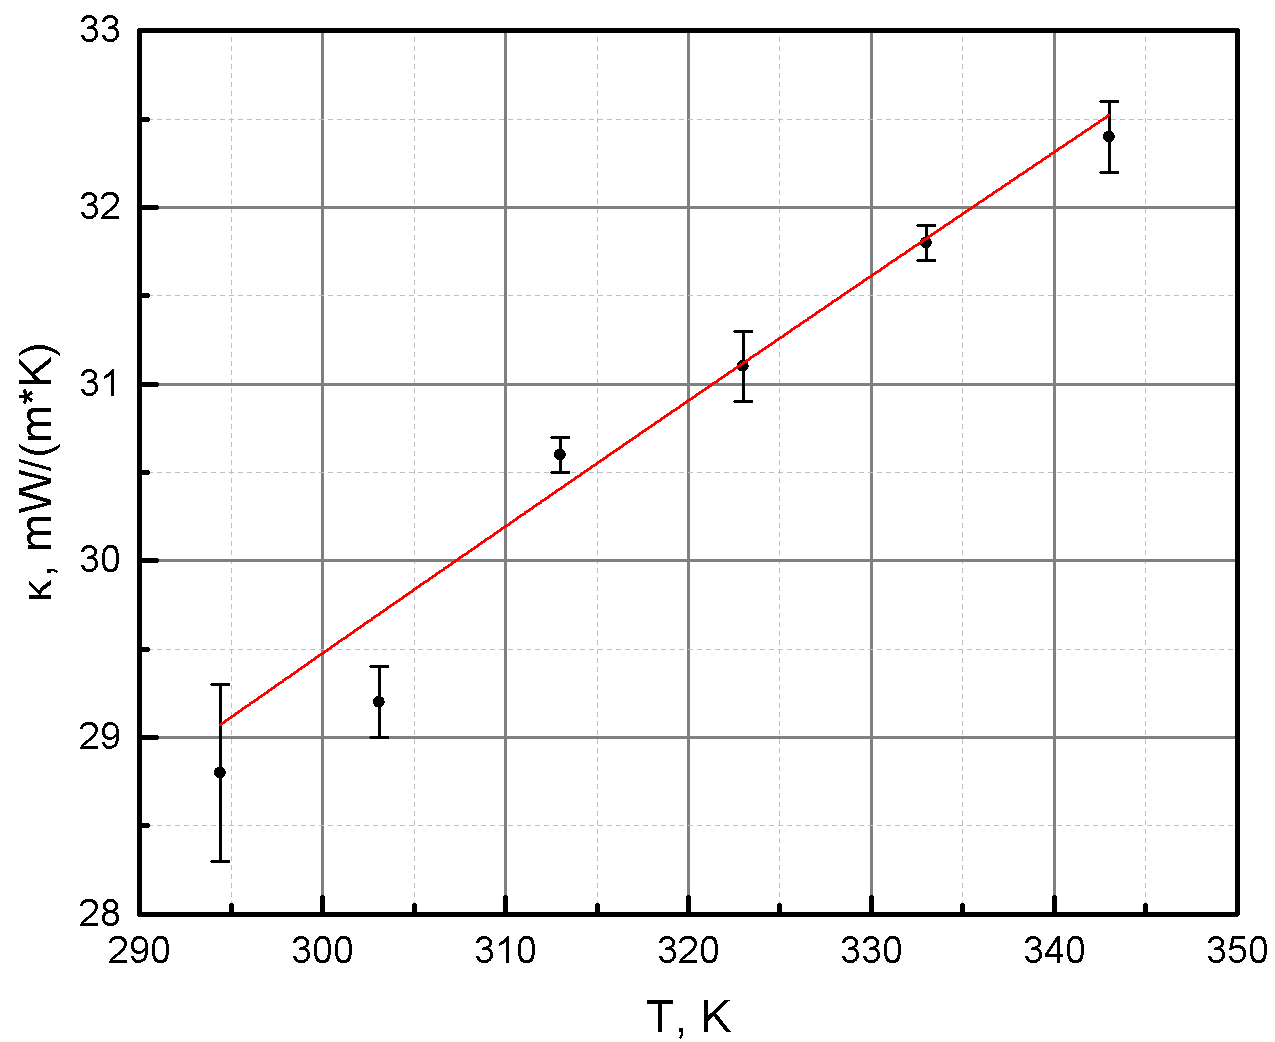
\includegraphics[width=8cm,height=7cm]{Graph_8_1}}
 \ffigbox[\FBwidth]{\caption{Зависимость $\ln {\varkappa/\varkappa_0}$ от $\ln {T/T_0}$.}\label{fig:Graph_8_2}}%
         {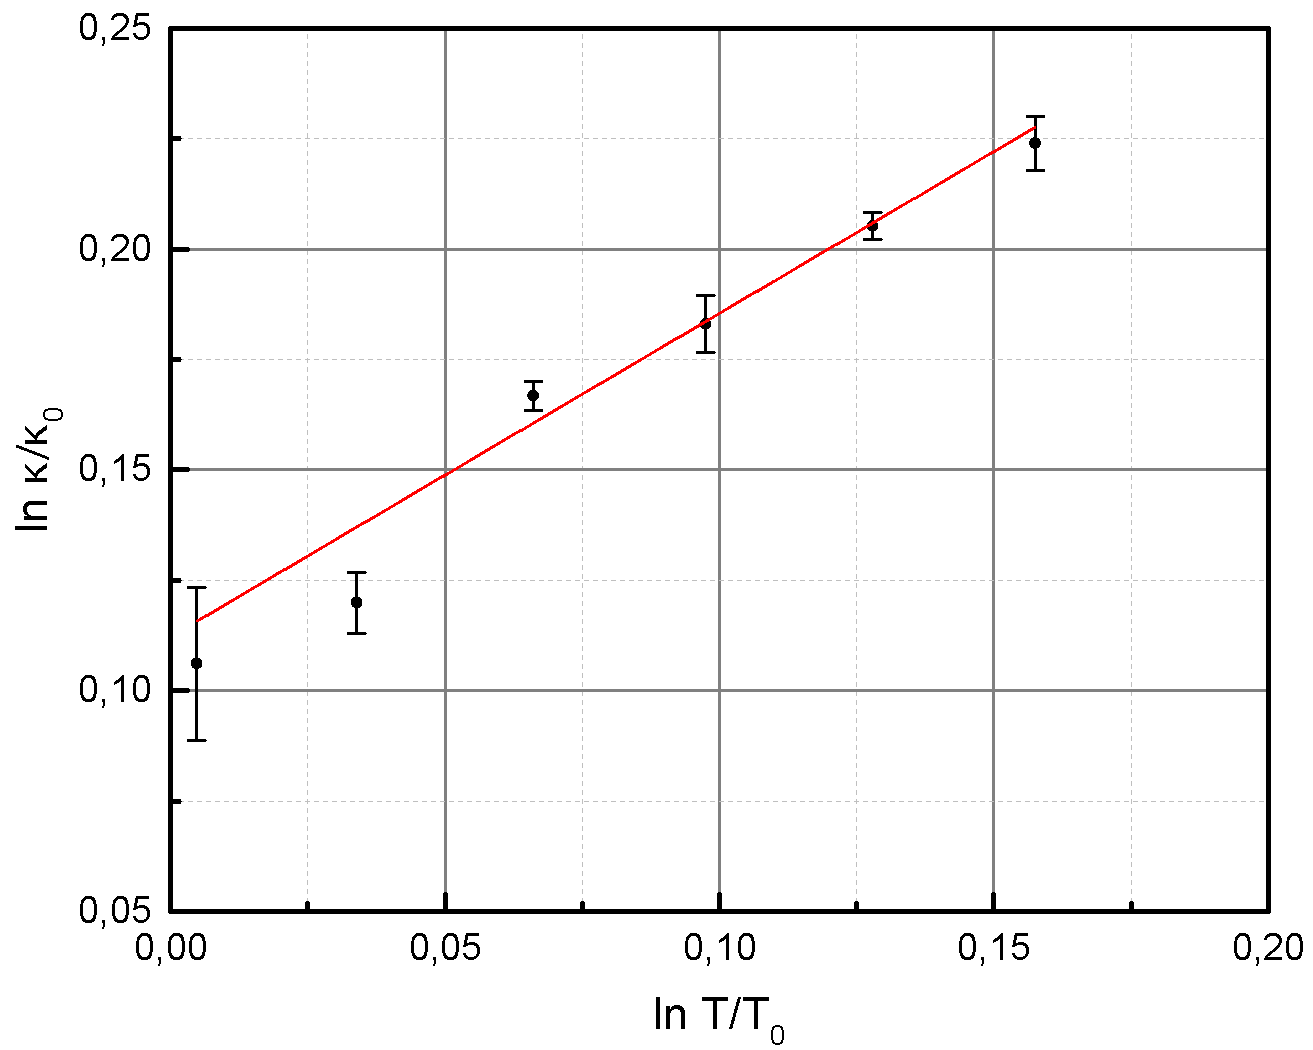
\includegraphics[width=8cm,height=7cm]{Graph_8_2}}         
\end{floatrow}
\end{figure}	
\end{enumerate}


\newpage
\section{Обсуждение результатов}
	В ходе данной работы мы определили коэффициент теплопроводности воздуха при атмосферном давлении и разных температурах по теплоотдаче нагреваемой током нити в цилиндрическом сосуде. В среднем каждое значение коэффициента теплопроводности отличается от табличного при данной температуре на 10\%. По полученным результатам рассчитали коэффициент $\beta$ в формуле $\varkappa = AT^\beta$: $\beta = 0,73 \pm 0,08$. Однако полученный результат с учетом погрешности не соотвествует теоретическому значению $\beta = 0,5$ ($\varkappa \propto \sqrt{T}$), то есть наш результат завышен на 46\%\footnote{Удивительно, что если построить аналогичным образом прямую, используя табличные значения коэффициента теплопроводности воздуха при атмосферном давлении, то $\beta = 0,81$, тогда в этом случае наш результат занижен на 10\%.}. Во-первых, это может быть связано с неучтенными тепловыми потерями через основания цилиндра. Во-вторых, количество экспериментальных точек достаточно мало. В-третьих, при выводе формулы (\ref{formula}) пренебрегалось зависимостью теплопроводности от температуры, поэтому она справедлива только при $\Delta T \ll T$. И наконец, возникновение термо-ЭДС (эффект Зеебека) повлияло на точность вольтметра. Стоит отметить, что крайняя левая экспериментальная точка на графике~\ref{fig:Graph_8_2} должна находиться вблизи точки (0, 0), то есть наша прямая смещена на некоторую константу от теоретичекой прямой, значит, в нашем эксперименте имеется неучтенная систематическая погрешность. 
	
	Для получения более точного результата необходимо увеличить диапазон рабочих температур, количество экспериментальных точек и уменьшить шаг изменения температуы.


\section{Выводы}


\begin{enumerate}
\item
	Определили коэффициент теплопроводности воздуха при атмосферном давлении и разных температурах по теплоотдаче нагреваемой током нити в цилиндрическому сосуде. Например при $T = 303$К: $\varkappa = (30,6 \pm 0,1)$ мВт/(м$\cdot$К).
	
\item
	В предположении, что $\varkappa = AT^\beta$, рассчитали коэффициент $\beta = 0,73 \pm 0,08$.
	
\item
	Предложили способы по улучшению точности определения коэффициента $\beta$.
\end{enumerate}
\end{document}
